\section{Eficiência e Viabilidade Industrial ($H_4$)}

A validação da Hipótese $H_4$ exige o equilíbrio entre o rigor estatístico e a viabilidade operacional. A Tabela \ref{tab:industrial_ranking} consolida os indicadores de produtividade para os modelos treinados na melhor versão do dataset (V10).

\begin{table}[!h]
    \centering
    \begin{threeparttable}
    \caption{Ranking de Eficiência Industrial (Dataset V10).}
    \label{tab:industrial_ranking}
    \begin{tabular}{llllll}
\toprule
Modelo & MCC & Parâmetros (M) & Tamanho (MB) & Latência (ms) & GFLOPs \\
\midrule
DENSENET & \textbf{0,6461} & 7,4838 & \textbf{29,1242} & 19,0448 & 2,8651 \\
CONVNEXT & 0,6153 & 28,3478 & 108,2258 & \textbf{6,4413} & 4,4702 \\
EFFICIENTNET & 0,5915 & 8,0643 & 31,2395 & 12,9784 & \textbf{0,6813} \\
VGG & 0,4910 & 33,0164 & 126,0395 & 11,2935 & 19,5511 \\
RESNET & 0,4501 & 24,6910 & 94,4991 & 7,8715 & 4,1106 \\
VIT & 0,4328 & 86,0297 & 328,2475 & 15,2857 & 16,8669 \\
SWIN & 0,4143 & 28,0470 & 107,2936 & 11,2551 & 4,5090 \\
INCEPTION & 0,2882 & 23,8940 & 91,4711 & 11,9814 & 2,8473 \\
\bottomrule
\end{tabular}

    \begin{tablenotes}
            \small 
            \item[] Fonte: Do autor.
        \end{tablenotes}
        \end{threeparttable}
\end{table}

Para visualizar o compromisso entre as métricas, a Figura \ref{fig:efficiency_tradeoff_full} apresenta o gráfico de dispersão correlacionando o MCC, a latência de inferência e a complexidade computacional (GFLOPs).

\begin{figure}[h!]
  \centering
  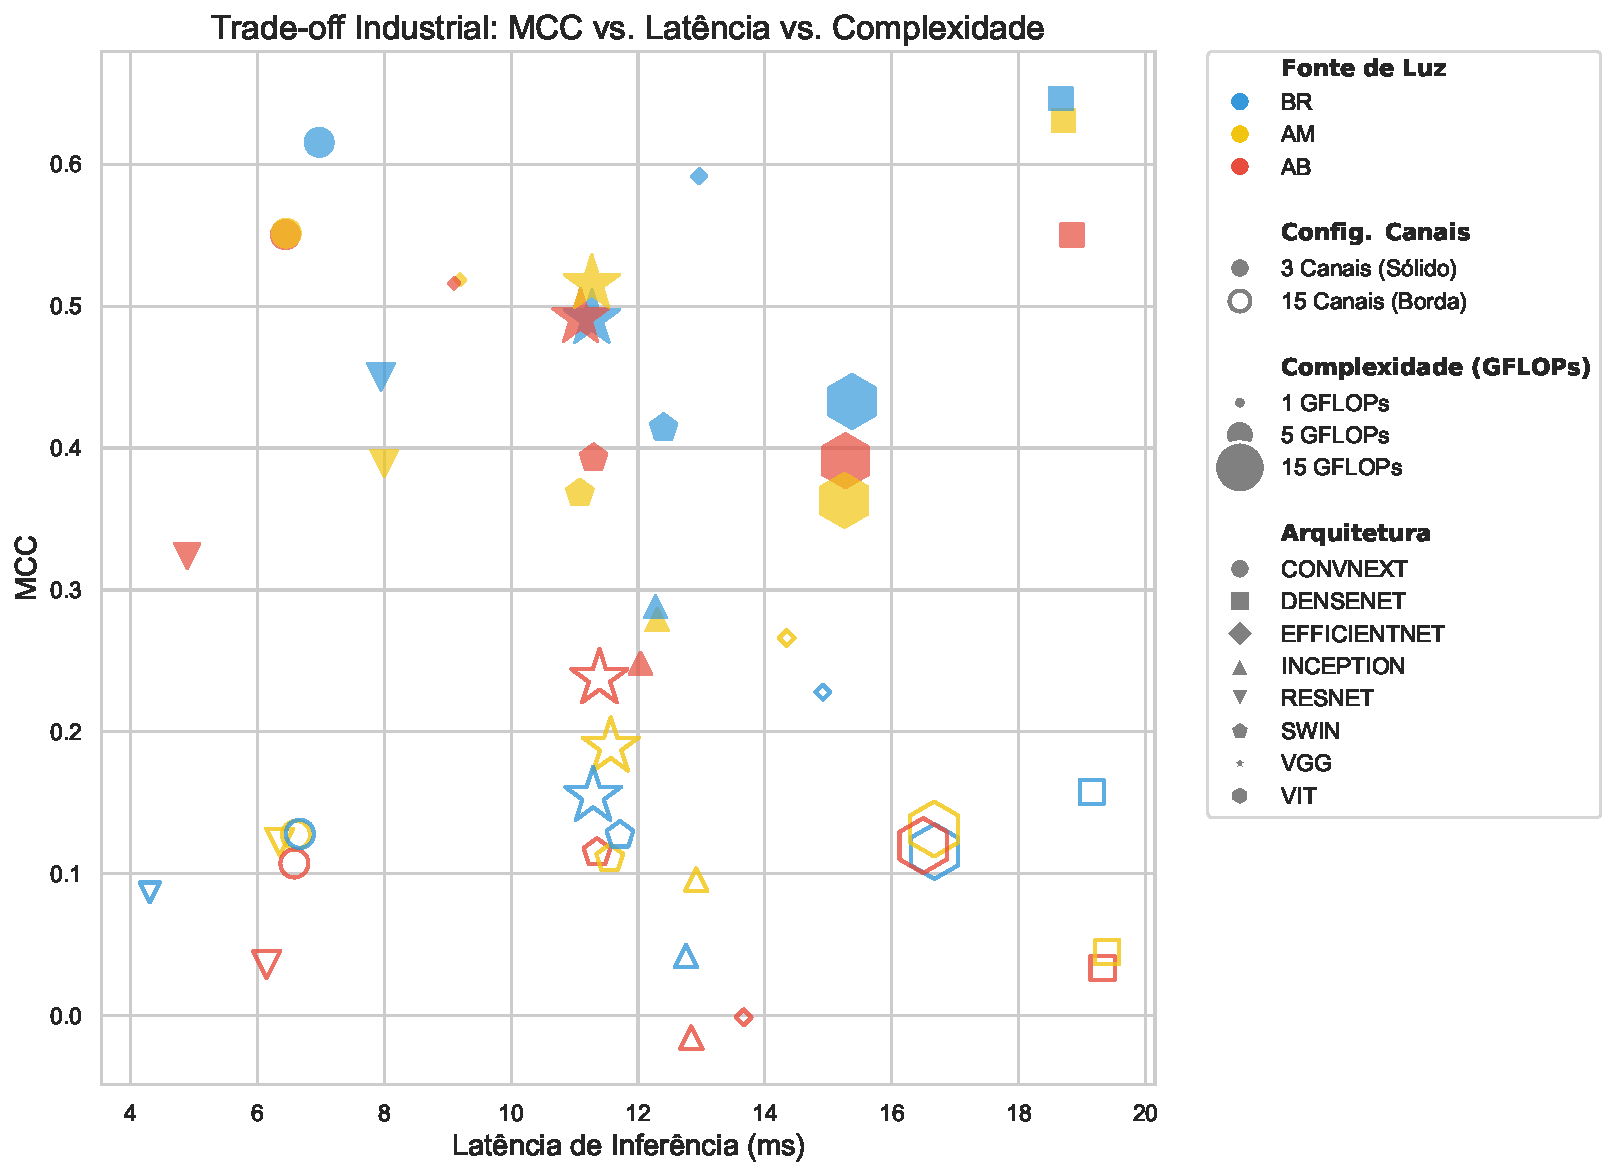
\includegraphics[width=1.0\textwidth]{images/efficiency_tradeoff_full.pdf}
  \caption{Trade-off Industrial: MCC vs. Latência (escala logarítmica). O tamanho das bolhas representa a complexidade em GFLOPs. Observa-se o agrupamento das CNNs modernas no quadrante superior esquerdo.}
  \label{fig:efficiency_tradeoff_full}
\end{figure}

A análise da Figura \ref{fig:efficiency_tradeoff_full} permite identificar três perfis tecnológicos distintos:
\begin{enumerate}
    \item \textbf{Alta Precisão (Elite):} A \textbf{DenseNet} ocupa o topo do eixo Y, mas desloca-se para a direita no eixo de latência, indicando um custo computacional elevado para o ganho marginal de performance.
    \item \textbf{Ponto de Operação Industrial (Sweet Spot):} A \textbf{ConvNext} situa-se no quadrante superior esquerdo, mantendo um MCC elevado com a menor latência entre os modelos de alta performance. O tamanho moderado de sua bolha (GFLOPs) reforça sua adequação para sistemas de tempo real.
    \item \textbf{Baixa Eficiência Relativa:} Os modelos baseados em \textbf{Transformers} (bolhas maiores e mais à direita) demonstram baixa eficiência para este problema específico, apresentando alta latência sem superar a barreira de performance das CNNs.
\end{enumerate}

Conclui-se que, embora a DenseNet possua superioridade estatística, a \textbf{ConvNext} emerge como a solução de maior viabilidade industrial, confirmando os pressupostos da hipótese $H_4$ ao oferecer o melhor balanço entre agilidade e assertividade.
